%!TEX root = ../../domainanalyse.tex
\chapter{Domain Modell}
	\section{Domain Modell}
		\subsection{Domain Modell}
			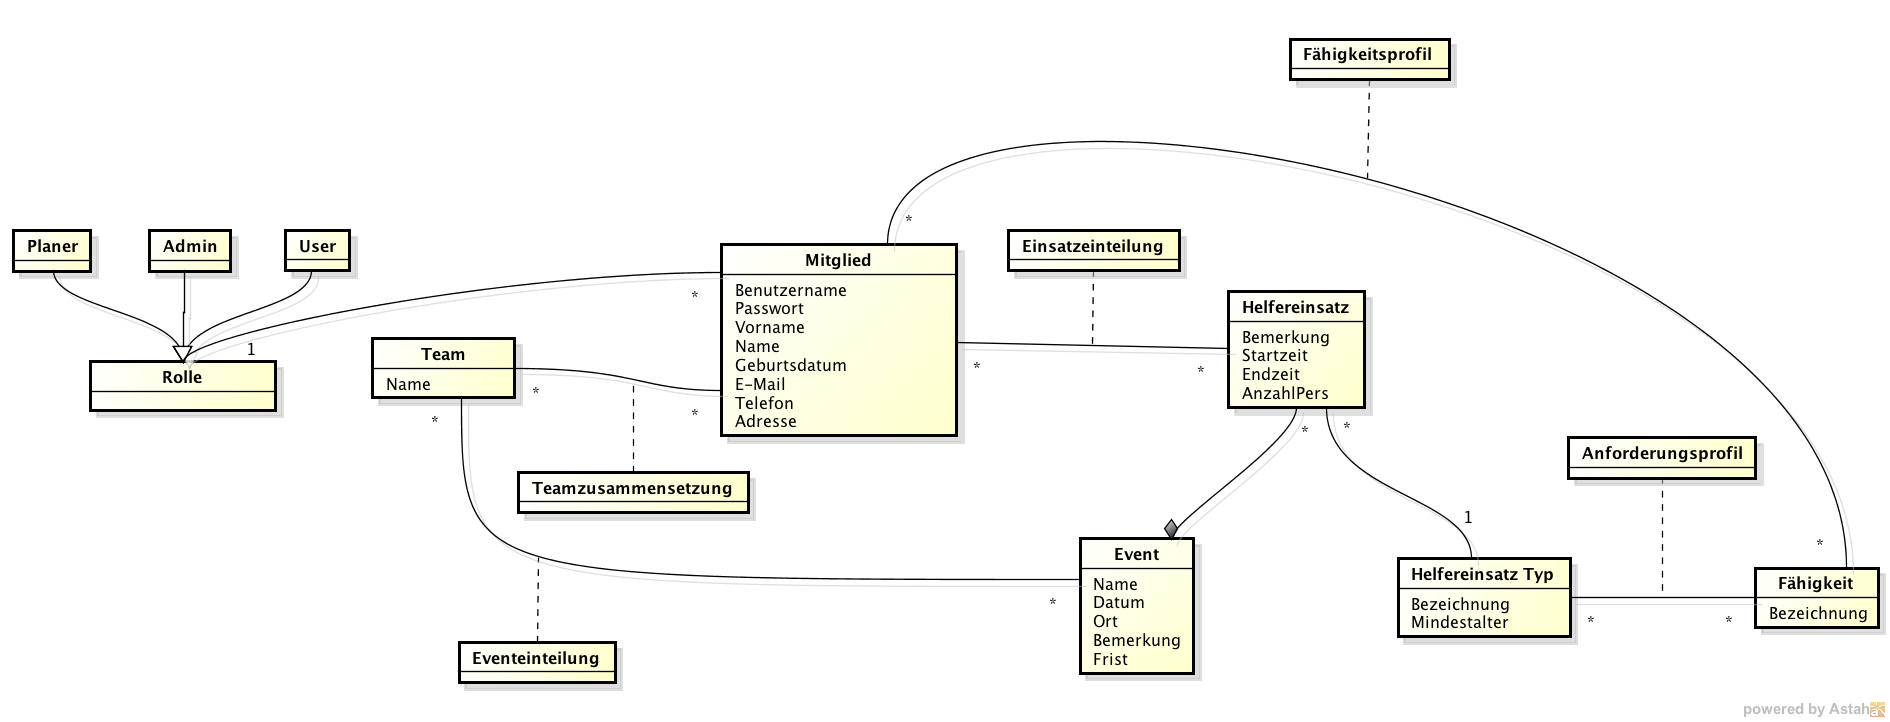
\includegraphics[width=\textwidth]{content/domainanalyse/images/Domainmodell_mit_Assoziationen.png}

	\section{Klassenspezifikation}
	\subsection{Event}
	Ein \underline{Event} stellt einen Anlass bzw. einen Spieltag dar, für den es Helfer braucht, um gewisse Aufgaben zu erledigen. Es gibt vor, welche Aufgaben (\underline{Helfereinsätze}) verteilt werden müssen und welche \underline{\underline{Mitglieder}} dazu in frage kommen. Letzteres geschieht über die Zuordnung von \underline{Teams}.

	\subsubsection*{Attribute}
    \begin{table}[H]
        \tablestyle
        \tablealtcolored
        \begin{tabularx}{\textwidth}{l l X}
        \tableheadcolor
            \tablehead Attribut & 
            \tablehead Typ & 
            \tablehead Beschreibung \tabularnewline  
        \tablebody
			Name      & String & Name des Events \tabularnewline                                                  
			Datum     & Date   & Durchführungsdatum \tabularnewline                                               
			Ort       & String & Freie Ortsangabe, ohne Adressformat \tabularnewline                              
			Bemerkung & String & Optionale Bemerkung zum Event. Kann längeren Text beinhalten. \tabularnewline    
			Frist     & Date   & Datum, ab welchem keine An- und Abmeldungen mehr zugelassen sind. \tabularnewline 
        \tableend
        \end{tabularx} 
    \end{table}

    \subsubsection*{Relationen}
    \begin{table}[H]
        \tablestyle
        \tablealtcolored
        \begin{tabularx}{\textwidth}{l l l X}
        \tableheadcolor
            \tablehead Nr & 
            \tablehead Klasse & 
            \tablehead Multiplizität & 
            \tablehead Beschreibung \tabularnewline  
        \tablebody
			1 & \underline{Helfereinsatz} & 1:n & Legt fest, welche Helfereinsätze zum Event gehören. \tabularnewline 
			2 & \underline{Team} & n:m & Dient dazu, Mitglieder für Helfereinsätze freizuschalten. Pro Event können mehrere Teams zuständig sein. \tabularnewline 
        \tableend
        \end{tabularx} 
    \end{table}

    \subsection{Mitglied}
    Ein \underline{Mitglied} stellt sowohl ein Mitglied des Vereins, als auch einen Benutzer des Systems dar. \underline{Mitglieder} werden für \underline{Helfereinsätze} eingeteilt.

    \subsubsection*{Attribute}
    \begin{table}[H]
        \tablestyle
        \tablealtcolored
        \begin{tabularx}{\textwidth}{l l X}
        \tableheadcolor
            \tablehead Attribut & 
            \tablehead Typ & 
            \tablehead Beschreibung \tabularnewline  
        \tablebody
			Benutzername & String  & Anmeldename für den Benutzer. \tabularnewline  
			Passwort     & String  & Zum Benutzernamen gehöriges Passwort für Anmeldung. \tabularnewline  
			Vorname      & String  & Vorname des \underline{Mitglieds} \tabularnewline  
			Name         & String  & Nachname des \underline{Mitglieds} \tabularnewline  
			Geburtsdatum & Date    & Geburtsdatum des \underline{Mitglieds} \tabularnewline  
			E-Mail       & String  & E-Mail Adresse des \underline{Mitglieds} \tabularnewline  
			Telefon      & String  & Optional: Telefonnummer des \underline{Mitglieds} \tabularnewline  
			Adresse      & Address & Wohnadresse/Anschrift des \underline{Mitglieds}. \tabularnewline  
        \tableend
        \end{tabularx} 
    \end{table}

    \subsubsection*{Relationen}
    \begin{table}[H]
        \tablestyle
        \tablealtcolored
        \begin{tabularx}{\textwidth}{l l l X}
        \tableheadcolor
            \tablehead Nr & 
            \tablehead Klasse & 
            \tablehead Multiplizität & 
            \tablehead Beschreibung \tabularnewline  
        \tablebody
			3 & \underline{Team}          & n:m & Beschreibt, welche \underline{Mitglieder} in welchen \underline{Teams} sind. Ein Mitglied kann auch zu mehreren \underline{Teams} gehören. \tabularnewline
			4 & \underline{Rolle}         & n:1 & Zuweisung von Rolle an \underline{Mitglieder}. \tabularnewline
			5 & \underline{Fähigkeit}     & n:m & Legt fest, welche Fähigkeiten ein \underline{Mitglied} besitzt. \tabularnewline
			6 & \underline{Helfereinsatz} & n:m & Zuordnung von Helfereinsätzen und \underline{Mitglieder}n. Damit die Verbindung zulässig ist, müssen \underline{Anforderungsprofil} und \underline{Fähigkeitsprofil} übereinstimmen. \tabularnewline
        \tableend
        \end{tabularx} 
    \end{table}

    \subsection{Team}
	Stellt eine Mannschaft des Vereins dar und kann einem \underline{Event} zugeordnet werden. Die dazugehörigen \underline{Mitglieder} werden somit für die \underline{Helfereinsätze} des \underline{Events} freigeschaltet.

    \subsubsection*{Attribute}
    \begin{table}[H]
        \tablestyle
        \tablealtcolored
        \begin{tabularx}{\textwidth}{l l X}
        \tableheadcolor
            \tablehead Attribut & 
            \tablehead Typ & 
            \tablehead Beschreibung \tabularnewline  
        \tablebody
			Name & String  & Name der Mannschaft. \tabularnewline 
        \tableend
        \end{tabularx} 
    \end{table}

    \subsubsection*{Relationen}
    \begin{table}[H]
        \tablestyle
        \tablealtcolored
        \begin{tabularx}{\textwidth}{l l l X}
        \tableheadcolor
            \tablehead Nr & 
            \tablehead Klasse & 
            \tablehead Multiplizität & 
            \tablehead Beschreibung \tabularnewline  
        \tablebody
			7 & \underline{Mitglied} & m:n & Inversion \#3 \tabularnewline  
			8 & \underline{Event}    & m:n & Inversion \#2 \tabularnewline  
        \tableend
        \end{tabularx} 
    \end{table}

    \subsection{Helfereinsatz Typ}
	Diese Klasse dient als Vorlage für \underline{Helfereinsätze}. Sie beschreibt eine gewisse Tätigkeit und definiert die Anforderungen (\underline{Fähigkeiten}), welche ein \underline{Mitglied} erfüllen muss, um sich für einen \underline{Helfereinsatz} dieses Typs anmelden zu können.

    \subsubsection*{Attribute}
    \begin{table}[H]
        \tablestyle
        \tablealtcolored
        \begin{tabularx}{\textwidth}{l l X}
        \tableheadcolor
            \tablehead Attribut & 
            \tablehead Typ & 
            \tablehead Beschreibung \tabularnewline  
        \tablebody
			Bezeichnung  & String  & Titel/Bezeichung des Typs \tabularnewline  
			Mindestalter & Integer & Mindestalter, welches ein \underline{Mitglied} haben muss, um sich für einen \underline{Helfereinsatz} dieses Typs anmelden zu können. \tabularnewline  
        \tableend
        \end{tabularx} 
    \end{table}

    \subsubsection*{Relationen}
    \begin{table}[H]
        \tablestyle
        \tablealtcolored
        \begin{tabularx}{\textwidth}{l l l X}
        \tableheadcolor
            \tablehead Nr & 
            \tablehead Klasse & 
            \tablehead Multiplizität & 
            \tablehead Beschreibung \tabularnewline  
        \tablebody
			9  & \underline{Helfereinsatz} & 1:n & Inversion von \#15 \tabularnewline
			10 & \underline{Fähigkeit}     & n:m & Definiert vorausgesetzte \underline{Fähigkeiten} für Typ \tabularnewline
        \tableend
        \end{tabularx} 
    \end{table}

    \subsection{Fähigkeit}
	Fähigkeiten/Kompetenzen, die \underline{Mitglieder} haben können, um sich dadurch für bestimmte \underline{Helfereinsätze} zu qualifizieren.

    \subsubsection*{Attribute}
    \begin{table}[H]
        \tablestyle
        \tablealtcolored
        \begin{tabularx}{\textwidth}{l l X}
        \tableheadcolor
            \tablehead Attribut & 
            \tablehead Typ & 
            \tablehead Beschreibung \tabularnewline  
        \tablebody
			Bezeichnung & String  & Titel/Bezeichung der \underline{Fähigkeit}. \tabularnewline
        \tableend
        \end{tabularx} 
    \end{table}

    \subsubsection*{Relationen}
    \begin{table}[H]
        \tablestyle
        \tablealtcolored
        \begin{tabularx}{\textwidth}{l l l X}
        \tableheadcolor
            \tablehead Nr & 
            \tablehead Klasse & 
            \tablehead Multiplizität & 
            \tablehead Beschreibung \tabularnewline  
        \tablebody
			11 & \underline{Helfereinsatz Typ} & 1:n & Inversion \#10 \tabularnewline  
			12 & \underline{Mitglied}          & m:n & inversion \#5 \tabularnewline  
        \tableend
        \end{tabularx} 
    \end{table}

    \subsection{Rolle}
    Definiert eine \underline{Rolle}, welche ein \underline{Mitglied} annehmen kann. Die zugewiesenen \underline{Rollen} nehmen Einfluss darauf, wie sich das System gegenüber dem \underline{Mitglied} verhält. 

    \subsubsection*{Relationen}
    \begin{table}[H]
        \tablestyle
        \tablealtcolored
        \begin{tabularx}{\textwidth}{l l l X}
        \tableheadcolor
            \tablehead Nr & 
            \tablehead Klasse & 
            \tablehead Multiplizität & 
            \tablehead Beschreibung \tabularnewline  
        \tablebody
			13 & \underline{Mitglied}          & 1:n & Inversion \#4 \tabularnewline
        \tableend
        \end{tabularx} 
    \end{table}

    \subsubsection*{Abgeleitete Klassen}
    \begin{table}[H]
        \tablestyle
        \tablealtcolored
        \begin{tabularx}{\textwidth}{l X}
        \tableheadcolor
            \tablehead Klasse &
            \tablehead Beschreibung \tabularnewline  
        \tablebody
			User   & Kann Einsatzeinteilung verwalten (beschränkt auf eigenes \underline{Mitglieds}objekt und \underline{Helfereinsätze}, welche einem \underline{Event} angehören, die einem \underline{Team} zugeordnet sind, in dem er selbst vorkommt). \tabularnewline
			Planer & Kann \underline{Event}, \underline{Helfereinsatz Typ}, \underline{Helfereinsatz}, \underline{Eventeinteilung}, \underline{Einsatzeinteilung} und \underline{Anforderungsprofil} verwalten. \tabularnewline
			Admin  & Alle Rechte von User und Planer. Zusätzlich kann ein Admin \underline{Mitglied}, \underline{Team}, \underline{Teamzusammensetzung} und \underline{Fähigkeitsprofil} verwalten. \tabularnewline
        \tableend
        \end{tabularx} 
    \end{table}

    \subsection{Helfereinsatz}
    Ein \underline{Helfereinsatz} stellt die Verbindung zwischen \underline{Helfereinsatz Typen} und \underline{Events} her. Objekte dieser Klasse besitzen Informationen zu den Details der Zuordnung.

    \subsubsection*{Attribute}
    \begin{table}[H]
        \tablestyle
        \tablealtcolored
        \begin{tabularx}{\textwidth}{l l X}
        \tableheadcolor
            \tablehead Attribut & 
            \tablehead Typ & 
            \tablehead Beschreibung \tabularnewline  
        \tablebody
			Bemerkung & String & Weitere Informationen in Textform. \tabularnewline
			Startzeit & Time   & Uhrzeit von Beginn des \underline{Helfereinsatz} \tabularnewline
			Endzeit   & Time   & Uhrzeit von Ende des \underline{Helfereinsatz} \tabularnewline
        \tableend
        \end{tabularx} 
    \end{table}

    \subsubsection*{Relationen}
    \begin{table}[H]
        \tablestyle
        \tablealtcolored
        \begin{tabularx}{\textwidth}{l l l X}
        \tableheadcolor
            \tablehead Nr & 
            \tablehead Klasse & 
            \tablehead Multiplizität & 
            \tablehead Beschreibung \tabularnewline  
        \tablebody
			14 & \underline{Event}             & n:1 & Inversion \#1 \tabularnewline
			15 & \underline{Helfereinsatz Typ} & n:1 & Definiert, auf welchem \underline{Helfereinsatz Typ} der \underline{Helfereinsatz} beruht. \tabularnewline
			16 & \underline{Mitglied}          & m:n & Inversion von \#6 \tabularnewline
        \tableend
        \end{tabularx} 
    \end{table}

    \subsection{Assoziationsklassen}
    \subsubsection*{Einsatzeinteilung}
		\begin{table}[H]
		    \tablestyle
		    \tablealtcolored
		    \begin{tabularx}{\textwidth}{l X l}
		        \tablebody
		        \tablehead Einsatzeinteilung &
					Speichert die Zuordnung von einzelnen \underline{Mitgliedern} und \underline{Helfereinsätzen}.
		        \tabularnewline
		        \tablehead Eventeinteilung &
					Stellt Verbindung zwischen \underline{Teams} und \underline{Events} her. Für ein \underline{Event} können mehrere \underline{Teams} zuständig sein.
		        \tabularnewline
		        \tablehead Fähigkeitsprofil &
					Legt fest, welche \underline{Fähigkeiten} ein \underline{Mitglied} besitzt.
		        \tabularnewline
		        \tablehead Anforderungsprofil &
					Bestimmt Voraussetzungen in Form von \underline{Fähigkeiten}, die für einen \underline{Helfereinsatz Typ} erfüllt werden müssen. 
		        \tabularnewline
		        \tablehead Teamzusammensetzung &
					Definiert, welche \underline{Mitglieder} in welche \underline{Teams} gehören. Ein \underline{Mitglied} kann somit mehreren \underline{Teams} angehören
		        \tabularnewline
		        \tableend
		    \end{tabularx}
		    \caption{Unit Testing}
		\end{table}
